
\documentclass[12pt]{book}

\usepackage[utf8]{inputenc}
\usepackage[greek, english]{babel}

% Packages
\usepackage{alphabeta}
\usepackage{amsmath}
\usepackage{amsthm}
\usepackage{caption}
\usepackage{color}
\usepackage{fullpage}
\usepackage{graphicx}
\usepackage{latexsym}
\usepackage{listings}
\usepackage{pxfonts}
\usepackage{stackrel}
\usepackage{titlesec}
\usepackage{subfig}
\usepackage{tikz}
\usepackage{float}
\usepackage{hyperref}
\usepackage{setspace}
\usepackage{hyperref}
\usepackage{tcolorbox}
\tcbuselibrary{theorems}

\newtcbtheorem[number within=section]{mytheorem}{Θεώρημα}%
{colback=black!5,colframe=black!15!black,fonttitle=\bfseries}{th}

% Commands
\newcommand{\N}{\mathbb{N}}
\newcommand{\R}{\mathbb{R}}
\newcommand{\code}[2]{\lstinputlisting[caption={#2}]{#1}}
\newcommand{\margin}{\hspace{4pt}}
\newcommand{\norm}[1]{\left\lVert#1\right\rVert}
\newcommand{\abs}[1]{\left\lvert#1\right\rvert}

% Environments
\newenvironment{matlab}
	{\begin{figure}[hp]\centering\captionsetup{justification=centering}}
	{\end{figure}}

\newenvironment{rcases}
	{\left.\begin{aligned}}
	{\end{aligned}\right\rbrace}

% Python Syntax Highlighting
\definecolor{string_color}{RGB}{0, 161, 13}
\definecolor{comment_color}{RGB}{46, 46, 46}
\definecolor{keyword_color}{RGB}{0, 112, 191}
\definecolor{background_color}{RGB}{250, 250, 250}

\lstset{
    framesep=15pt,
    xleftmargin=15pt,
    xrightmargin=15pt,
    language=Python,
    captionpos=b,
    numbers=right,
    numberstyle=\small\ttfamily,
    frame=lines,
    showspaces=false,
    showtabs=false,
    breaklines=true,
    showstringspaces=false,
    breakatwhitespace=true,
    commentstyle=\color{comment_color}\textit,
    keywordstyle=\bfseries\color{keyword_color}\textbf,
    stringstyle=\color{string_color}\textit,
    morekeywords={self, lambda, __init__, __del__, __name__, for, in, not, and, or, :},
    basicstyle=\small\ttfamily,
    tabsize=4,
    keepspaces=true,
    columns=flexible,
    backgroundcolor=\color{background_color}
}

% Links
\hypersetup{
    colorlinks=true,
    linkcolor=blue,
    filecolor=magenta,
    urlcolor=cyan,
}

% Lengths
\setlength{\parindent}{0in}
\setlength{\oddsidemargin}{0in}
\setlength{\textwidth}{6.5in}
\setlength{\textheight}{10in}
\setlength{\topmargin}{-1.0in}
\setlength{\headheight}{18pt}
\setlength{\parskip}{0.3cm}
\setlength{\parindent}{5ex}
\doublespacing

\theoremstyle{definition}
\newtheorem{definition}{Definition}[section]

\titlespacing*{\subsection}
{0pt}{5.5ex plus 1ex minus .2ex}{4.3ex plus .2ex}

\title{\huge Sudoku}
\author{Σιώρος Βασίλειος\\Ανδρινοπούλου Χριστίνα}
\date{Ιανουάριος 2020}

\begin{document}

\maketitle

\pagenumbering{gobble}
\pagebreak

\tableofcontents

\chapter{Abstract}

Το SUDOKU είναι ένα ιδιαίτερα δημοφιλές παιχνίδι, το οποίο έχει φανατικούς παίκτες σε όλον τον κόσμο, ανεξάρτητα ηλικιακής ομάδας, κοινωνικής τάξης ή άλλων χαρακτηριστικών. Πρόκειται για ένα παζλ βασιμένο στη λογική. \par

Στόχος του παιχνιδιού αυτού είναι ο παίκτης να συμπληρώσει τα
κενά κελιά ενός ημιτελώς συμπληρωμένου πίνακα μεγέθους
\(n \times n\) με τους κατάλληλους ακεραίους που ανήκουν στο διάστημα \(\left[1,\dots,n \right]\), με τέτοιον τρόπο ώστε κάθε γραμμή, κάθε στήλη και κάθε υποπίνακας μεγέθους \(m \times m\) να περιέχει όλους τους ακεραίους του διαστήματος  \(\left[1,\dots,n \right]\) ακριβώς μία φορά τον καθέναν. \par

Η πιο συνηθισμένη εκδοχή του SUDOKU είναι παζλ με πίνακα μεγέθους \(\left[9 \times 9\right]\) (ένα τέτοιο παράδειγμα παρατίθενται στο Figure 1.1), ωστόσο υπάρχουν και άλλες παραλλάγες του κλασσικού \(\left[9 \times 9\right] \) SUDOKU οι οποίες προκύπτουν με παραμετροποίηση του κλασσικού προτύπου SUDOKU, αλλά και προσθήκη επιπλέον περιορισμών που κάνουν την επίλυση του παζλ ακόμα πιο ενδιαφέρουσα. Σε αυτές θα αναφερθούμε εκτενώς στη συνέχεια. \par

Καθώς ο στόχος του παιχνιδιού δεν είναι μαθηματικής φύσης, η συμπλήρωση αριθμών στα κενά κελιά είναι καθαρά συμβολική. Οι αριθμοί μπορούν πολύ εύκολα να αντικατασταθούν με οποιαδήποτε ομάδα συμβόλων επιθυμεί κανείς, χωρίς να προκαλέσουν καμμία επίπτωση στην επίλυση, στη δημιουργία ή στη μαθηματική μοντελοποίηση του παζλ. Ήδη υπάρχουν διαθέσιμα SUDOKU παζλ με βάση κινέζικα σύμβολα, κινέζικους αριθμούς και σύμβολα που αναπαριστούν μερίδες σούσι. Φυσικά, αυτές οι παραλλαγές είναι ανεξάντλητες και ταυτόχρονα μηδαμινής σημασίας, γι'αυτό και δε θα επεκταθούμε περισσότερο σε αυτές. 

\begin{figure}[h]
	\centering	
	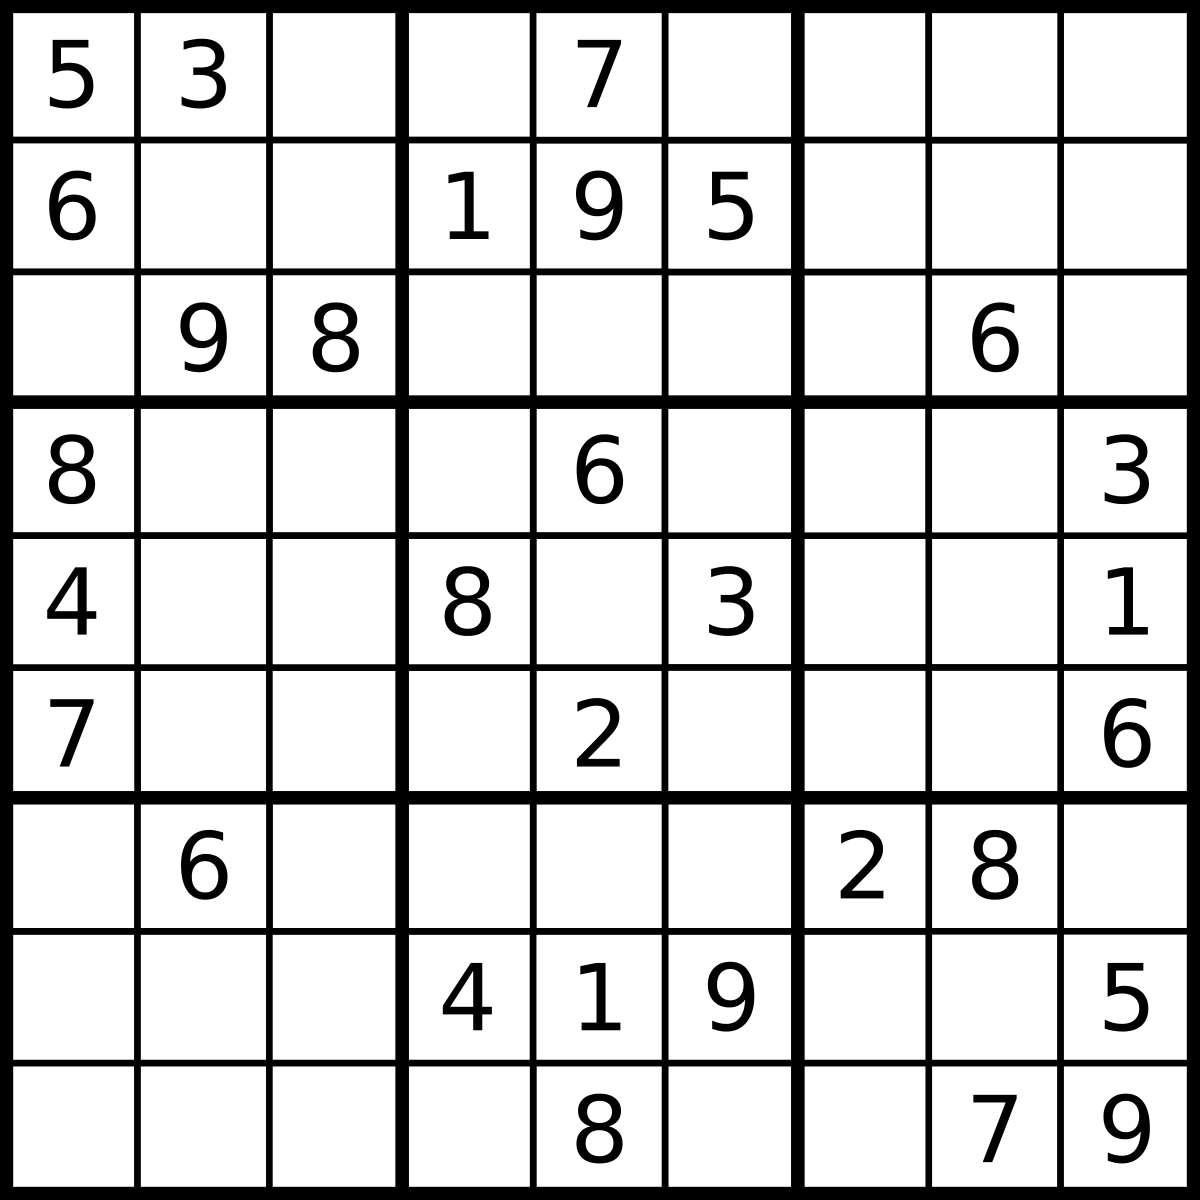
\includegraphics[scale=0.2]{Figures/classicSUDOKU.jpeg}
	\caption{Παράδειγμα κλασσικού SUDOKU \( 9 \times 9\) }
\end{figure}

\chapter{Ιστορικά στοιχεία}

Το SUDOKU, στη μορφή που το γνωρίζουμε, δημιουργήθηκε το 1979 από τον Αμερικανό αρχιτέκτονα Howard Garns (Figure 2.1). O Howard Garns \cite{1} γεννιέται τον Μάρτιο του 1905 στο Connersville του Indiana. Το 1922 αποφοιτεί από το Indianapolis Technical High School και τέσσερα χρόνια μετά αποκτά Bachelor στο Science in architectural engineering. Πεθαίνει από καρκίνο τον Οκτώβρη του 1989.  \par

\begin{figure}[h]
	\centering	
	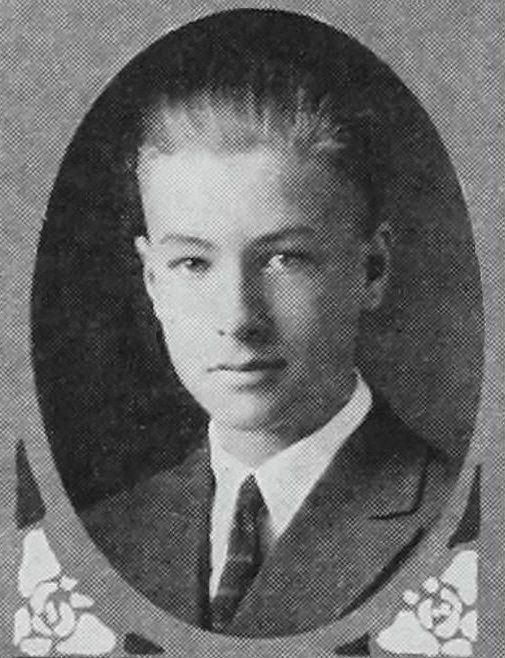
\includegraphics[scale=0.3]{Figures/Howard Garns.jpeg}
	\caption{ο Howard Garns υπήρξε ο δημιουργός του SUDOKU το 1979}
\end{figure}

Το παιχνίδι αρχικά ονομάστηκε “Number Place”, καθώς απαιτούσε την τοποθέτηση αριθμών στα κενά κελιά ενός πίνακα και
δημοσιεύτηκε στο περιοδικό Dell Pencil Puzzles and Word
Games το 1979. \par

Ενα χρόνο μετά το παιχνίδι έγινε ιδιαίτερα δημοφιλές στην Ιαπωνία και μετονομάστηκε σε “suji wa dokushin ni
kagiru”(SUDOKU), που σημαίνει ότι "τα ψηφία είναι περιορισμένα σε κάποιο κανόνα". \par

Το SUDOKU έγινε ιδιαίτερα αγαπητό στην Ιαπωνία, με τις μηνιαίες πωλήσεις SUDOKU περιοδικών να ανέρχονται στα
600.000 αντίτυπα κάθε μήνα.
Οι Ιάπωνες υιοθέτησαν το SUDOKU ως συνήθεια για δύο
βασικούς λόγους. Ο πρώτος λόγος έχει να κάνει με τη γλώσσα τους. Η γλώσσα τους δεν ήταν κατάλληλη, όπως άλλες γλώσσες σαν την ελληνική, για την ανάπτυξη σταυρόλεξων, οπότε υστερούσαν σε τέτοιου είδους παιχνίδια. Ο δεύτερος λόγος σχετίζεται με τις συνήθειες των κατοίκων της Ιαπωνίας, οι οποίοι συνηθίζουν να μετακινούνται σε καθημερινή βάση με τρένα και λεωφορεία και με αυτόν τον τρόπο διανύουν μεγάλες αποστάσεις και περνούν πολύ από τον χρόνο τους σε καθημερινή βάση μέσα σε μέσα μαζικής μεταφοράς. Συνεπώς, η ύπαρξη ενός τέτοιου παιχνιδιού έκανε τις χρονοβώρες μετακινήσεις τους πιο ευχάριστες και επικοδομητικές. \par 

\begin{figure}[h]
	\centering	
	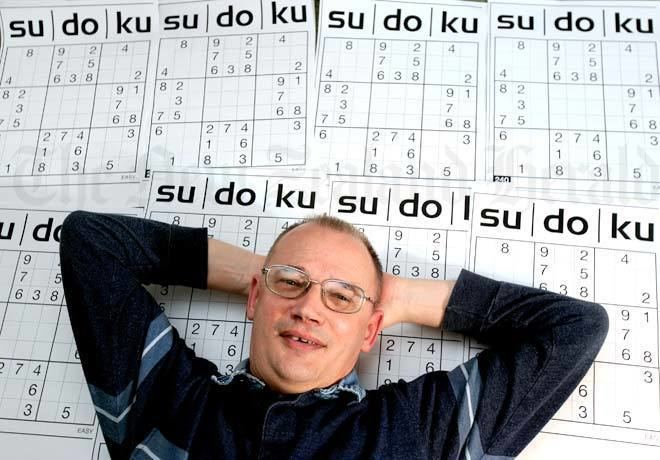
\includegraphics[scale=0.45]{Figures/WayneGould.jpg}
	\caption{ο Wayne Gould έκανε και πάλι αγαπητό το SUDOKU στη Δύση}
\end{figure}

Ο άνθρωπος που έφερε πίσω στον Δυτικό κόσμο το SUDOKU ήταν ο Wayne Gould (Figure 2.2). Ο Νεοζηλανδός Wayne Gould γεννήθηκε στις 3 Ιουλίου 1945 και υπήρξε δικαστής. Ωστόσο, εκείνο που τον έκανε ιδιαίτερα διάσημο δεν ήταν οι δικαστικές του ικανότητες, αλλά το γεγονός ότι έκανε το SUDOKU γνωστό στον Δυτικό κόσμο. Το 1997 βρισκόταν στο Τόκιο και ανακάλυψε ενα SUDOKU σε κάποιο βιβλιοπωλείο. Η ιδέα αυτού του παιχνιδιού τον ενθουσίασε ιδιαιτέρως. Μερικά χρόνια αργότερα έφτιαξε το πρωτο πρόγραμμα που δημιουργούσε SUDOKU παζλ διαφορετικών επιπέδων δυσκολίας. Ο Wayne Gould καταφέρνει τον Νοέμβριο του 2004 να πείσει το "The Times" στον Λονδίνο να δημοσιεύσουν ένα παζλ SUDOKU. Έπειτα από εκείνη τη δημοσίευση, ο κόσμος αγκάλιασε το παιχνίδι αυτό και για πολλούς ανθρώπους ανά τον κόσμο έγινε αγαπημένη συνήθεια.

\chapter{Εισαγωγή}

Το SUDOKU είναι ένα παζλ βασιμένο στη λογική. Στόχος του παιχνιδιού αυτού είναι η συμπλήρωση των
κενών κελιών ενός ημιτελώς συμπληρωμένου πίνακα μεγέθους
\(n \times n\) με τους κατάλληλους ακεραίους που ανήκουν στο διάστημα \(\left[1,\dots,n \right]\), με τέτοιον τρόπο ώστε κάθε γραμμή, κάθε στήλη και κάθε υποπίνακας μεγέθους \(m \times m\), όπου \(m = \sqrt{n} \) και \( m \ge 0\), να περιέχει όλους τους ακεραίους του διαστήματος  \(\left[1,\dots,n \right]\) ακριβώς μία φορά τον καθέναν. \par

\begin{mytheorem}{SUDOKU}{}
	Οι κανόνες για το κλασσικό SUDOKU σε έναν πίνακα μεγέθους \(n \times n\) με υποπίνακες μεγέθους \(m \times m\), 	όπου \(m = \sqrt{n}\) είναι: \\
	\(\bullet\) Κάθε γραμμή του πίνακα μεγέθους n να περιέχει ακριβώς μια φορά κάθε ακέραιο αριθμό από το 1 ως το n. \\
	\(\bullet\) Κάθε στήλη του πίνακα μεγέθους n να περιέχει ακριβώς μια φορά κάθε ακέραιο αριθμό από το 1 ως το n. \\
	\(\bullet\) Κάθε υποπίνακας μεγέθους \(m \times m\) να περιέχει ακριβώς μια φορά κάθε ακέραιο αριθμό από το 1 ως το n. \\
\end{mytheorem}

Το επίπεδο δυσκολίας από παζλ σε παζλ διαφέρει και σχετίζεται με την ποσότητα των συμπληρωμένων κελιών, αλλά και με τη θέση τους μέσα στο παζλ. \par

Η μελέτη μας θα εστιάσει στις μαθηματικές μεθοδολογίες για την επίλυση SUDOKU παζλ και στις μαθηματικές τεχνικές για τη δημιουργία SUDOKU παζλ. \par 

Κατά την παρουσίαση των μαθηματικών μεθοδολογιων που επιλύουν παζλ SUDOKU θα παρουσιάσουμε τη μοντελοποίηση του προβλήματος της επίλυσης του παζλ ως
πρόβλημα γραμμικού προγραμματισμού, έπειτα την επαλήθευση με χρήση MATLAB που έχει γίνει και τέλος θα αναφερθούμε σε ενδιαφέρουσες παραλλαγές του κλασσικού SUDOKU. \par

Στο κεφάλαιο που αφορά τις μαθηματικές τεχνικές για τη δημιουργία παζλ SUDOKU θα μελετήσουμε αρχικά την κατασκευή SUDOKU με bruteforce κι έπειτα θα εστιάσουμε στην κατασκευή SUDOKU με βάση παλαιότερα παζλ. \par

\chapter{Μελέτη των επιπέδων δυσκολίας στην επίλυση SUDOKU παζλ από τον άνθρωπο}

Στο παρόν κεφάλαιο θα μελετήσουμε τις τεχνικές που χρησιμοποιούνται από τον άνθρωπο για την επίλυση ενός SUDOKU παζλ και θα επιχειρήσουμε να μετρήσουμε τα επίπεδα δυσκολίας ενός τέτοιου παζλ. Δεν έχουν αναπτυχθεί ακόμη εφαρμόσιμες θεωρίες, που μπορούν να βοηθήσουν προς αυτήν την κατεύθυνση. Χωρίς βλάβη της γενικότητας στο κεφάλαιο αυτό όποτε αναφερόμαστε σε παζλ SUDOKU θα εννοούμε μεγέθους \(4 \times 4\), γιατί διευκολύνει τη μελέτη μας, εκτός αν αναφέρεται ρητά κατί διαφορετικό. \par

Το ζήτημα του προσδιορισμού των επιπέδων δυσκολίας για παζλ SUDOKU απασχολεί όχι μόνο τους δημιουργούς αυτών των παζλ, αλλά και τους ίδιους του παίκτες. Πώς ακριβώς προσδιορίζεται το επίπεδο δυσκολίας ενός παζλ; Μέχρι και σήμερα δεν υπάρχουν θεωρητικές προσεγγίσεις στις οποίες μπορούμε να βασιστούμε με σιγουριά για να απαντήσουμε το συγκεκριμένο ερώτημα. \par 

Σύμφωνα με τη μελέτη \cite{5} υπάρχουν δύο προσεγγίσεις του προβλήματος. Η πρώτη έχει να κάνει με την πολυπλοκότητα των ανεξάρτητων βημάτων που οδηγούν στη λύση του παζλ. Αυτή είναι η πιο συνηθισμένη προσέγγιση που χρησιμοποιείται για την εκτίμηση του επιπέδου δυσκολίας των παζλ. Η δεύτερη σχετίζεται με το αν τα βήματα που οδηγούν στη λύση είναι ανεξάρτητα ή οχι. \par

Θα ορίσουμε το πρόβλημα επίλυσης SUDOKU παζλ ως πρόβλημα ικανοποίησης περιορισμών, απόφαση που θα ερμηνευτεί λεπτομερέστερα σε επόμενο κεφάλαιο. Υπάρχουν δύο προσεγγίζεις για την επίλυση ενός προβλήματος απόφασης για SUDOKU παζλ, η backtracking και η constraint propagation. \par

Το backtracking είναι ουσιαστικά ένας bruteforce τρόπος επίλυσης προβλημάτων περιορισμών. Ξεκινά με μία κενή ανάθεση τιμών στις μεταβλητές τους προβλήματος και αναθέτοντας τιμές τη μία μετά την άλλη επιχειρεί να καταλήξει σε λύση. \par

Παζλ μεγέθους \(9 \times 9\) ο υπολογιστής είναι σε θέση να τα επιλύει με αυτήν την τεχνική σχετικά εύκολα. Ωστόσο, για τον άνθρωπο αυτή η προσέγγιση είναι ιδιαίτερα κουραστική και σίγουρα καθόλου διασκεδαστική, γι'αυτο και δεν προτιμάται σε καμμία περίπτωση. \par

\begin{figure}[h]
	\centering	
	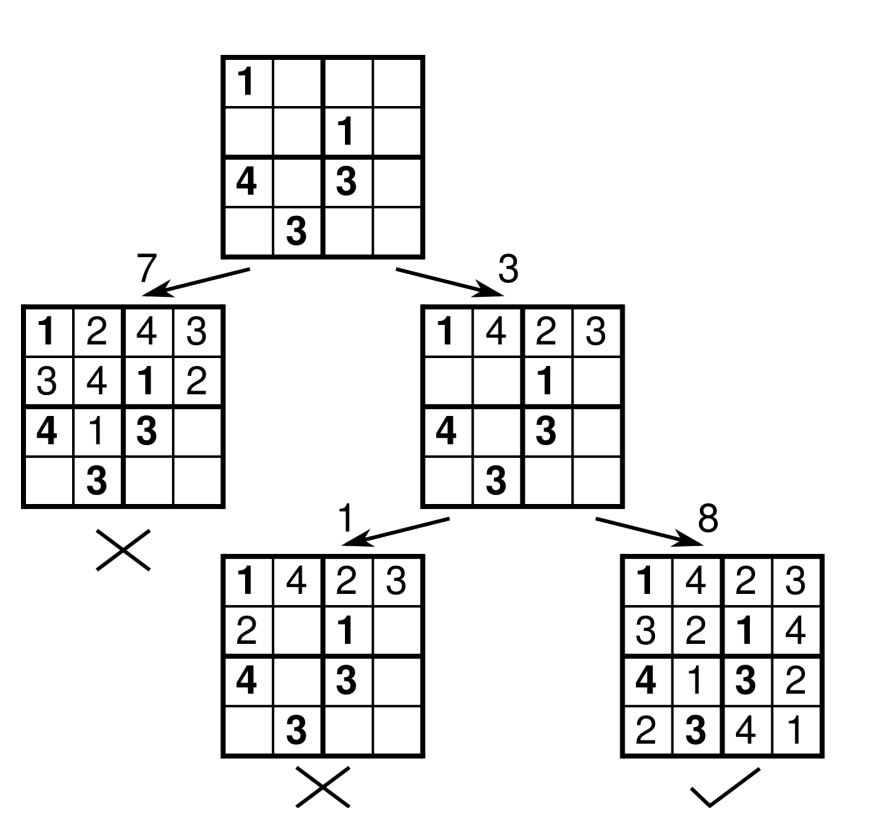
\includegraphics[scale=0.45]{Figures/backtracking.png}
	\caption{Μέρος της διαδικασίας επίλυσης ενός \(4 \times 4\) SUDOKU με την τεχνική backtracking}
\end{figure}

Με την constraint propagation τεχνική χρησιμοποιούμε τη λογική για να για να βρούμε την τιμή κάποιων μεταβλητών, εξετάζοντας τους περιορισμούς. Για κάθε μεταβλητή ορίζουμε ένα σύνολο τιμών που μπορεί να λάβει χωρίς να προκαλέσει την παραβίαση κανενός περιορισμού. \par

Η τεχική αυτή δεν είναι βέβαιο πως θα οδηγήσει σε λύση, αλλά σίγουρα είναι πιο αποδοτική. Μπορεί να συνδυαστεί με backtracking για καλύτερα αποτελέσματα. Το constraint propagation είναι η τεχνική που χρησιμοποιεί ο ανθρώπινος εγκέφαλος για να επιλύσει ένα SUDOKU παζλ. \par

\begin{figure}[h]
	\centering	
	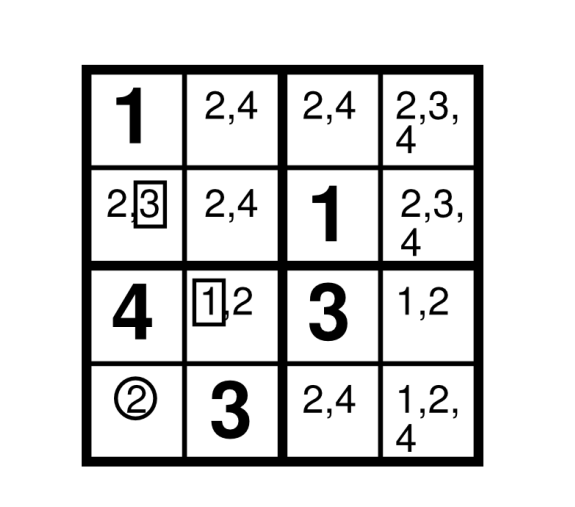
\includegraphics[scale=0.45]{Figures/propagation.png}
	\caption{Μέρος της διαδικασίας επίλυσης ενός \(4 \times 4\) SUDOKU με την τεχνική constraint propagation}
\end{figure}

Συγκεκριμένα ο άνθρωπος χρησιμοποιεί δύο είδη τεχνικών για να επιλύσει το παζλ: η Naked single technique (ή αλλιώς singleton, single value, forced value, exclusion
principle), όπου για ένα δεδομένο κελί του πίνακα υπάρχει μόνο μία τιμή που μπορεί να ανατεθεί, καθώς όλες οι υπόλοιπες τιμές πλήττουν κάποιον περιορισμο και η Hidden single technique (ή αλλιώς naked value, inclusion principle), όπου για μία συγκεκριμένη γραμμή ή στήλη ή για έναν συγκεκριμένο υποπίνακα του παζλ υπάρχει μόνο ένα κελί που μπορεί να φιλοξενήσει μία συγκεκριμένη τιμή. \par

Το πείραμα που πραγματοποιήθηκε για να συσχετίσει τη συμπεριφορά των ανθρώπων απέναντι σε παζλ, ώστε να προκύψουν συμπεράσματα για τα επίπεδα δυσκολίας τους στο \cite{5} αντλεί δεδομένα από τον παγκόσμιο ιστό. Καθώς το SUDOKU είναι ένα ευρέως διαδεδομένο παιχνίδι, υπάρχει πληθώρα δεδομένων στον παγκόσμιο ιστό που με κατάλληλη επεξερασία φάνηκαν χρήσιμα στην έρευνα. Φυσικά, τέτοια δεδομένα δεν είναι τα πλέον κατάλληλα, καθώς δεν υπόκεινται σε εργαστηριακόυς κανόνες, ωστόσο η πληθώρα τους τα κάνει εξίσου σημαντικά. \par

Ως μέτρο για την εκτίμηση την δυσκολίας των ανθρώπων να λύσουν ένα παζλ SUDOKU χρησιμοποιήθηκε ο μέσος χρόνος επίλυσης.

Αν πρέπει να ορίσουμε λίγο πιο αυστηρά το μοντέλο που χρησιμοποιεί ο άνθρωπος για την επίλυση SUDOKU, πρέπει να γίνουν ορισμένες παραδοχές. Ο άνθρωπος δεν είναι καλός στη συστηματική αναζήτηση, γι'αυτό και τεχνικές όπως το backtracking δεν τις προτιμα, όπως αναφέραμε προηγουμένως. Προτιμά να λύνει τέτοιου είδους προβλήματα με όσο το δυνατό πιο απλές λογικές τεχνικές όπως το constrait propagation. Επίσης, πρέπει να υποθέσουμε ότι κατά τη διαδικασία την επίλυσης του παζλ δε συμβαίνουν λάθη και ότι πάντα μπορεί να υπάρξει και επόμενο βήμα, μέχρι να φτάσουμε στη λύση. \par 

Το ανθρώπινο μοντέλο επίλυσης SUDOKU δίνεται παρακάτω: 

\begin{mytheorem}{Επίλυση SUDOKU από τον άνθρωπο}{}
	\(\bullet\) L είναι η πιο απλή τεχνική που μπορεί να προκαλέσει θετική έκβαση στην επίλυση του παζλ. \\
	\(\bullet\) Επιλογή του τρόπου (αν υπάρχουν πολλοί) που θα εφαρμοστεί το L στην τρέχουσα κατάσταση. \\
	\(\bullet\) Εφαρμογή. \\
\end{mytheorem}

Η αξιολόγηση του μοντέλου έγινε συγκρίνοντας τα δεδομένα των ανθρώπων που προέρχονταο από τον παγκόσμιο ιστό και τα δεδομένα από το μοντέλο. Χρησιμοποιήθηκαν 15 διαφορετικής δυσκολίας παζλ και κάθε παζλ επιλύθηκε από 10 εως και 60 άτομα. Τα αποτελέσματα αυτή της συσχέτισης φαίνονται στο Figure . \par

\begin{figure}[h]
	\centering	
	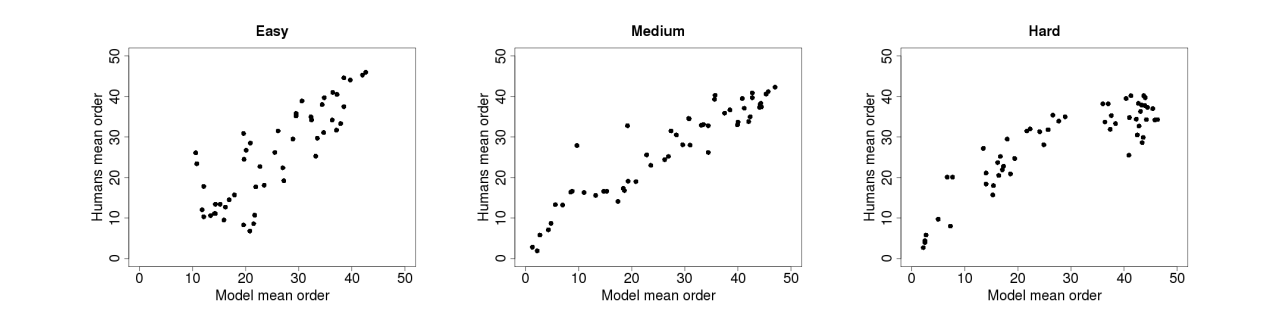
\includegraphics[scale=0.4]{Figures/results.png}
	\caption{Αποτελέσματα του πειράματος \cite{5}}
\end{figure}

Τελικά, η έρευνα \cite{5} καταλήγει στο συμπέρασμα ότι μπορούμε να βρούμε αρκετά καλές μετρικές για τα επίπεδα δυσκολίας ενός SUDOKU, ειδικά αν στη μοντελοποίηση λάβουμε υπόψη και ειδικά θέματα που σχετίζονται αποκλειστικά και μόνο με το SUDOKU ως παιχνίδι. 

\chapter{Επίλυση SUDOKU παζλ}
\section{Μαθηματική μοντελοποίηση}

Στο κεφάλαιο αυτό θα παρουσιάσουμε μία μαθηματική μοντελοποίηση του προβλήματος της επίλυσης των παζλ SUDOKU. Σκοπός του παρόντος κεφαλαίου είναι να προτείνουμε μια μαθηματική μοντελοποίηση που θα καθιστά δυνατή την εύρεση της λύσης του παζλ, αν υπάρχει, από έναν μαθηματικό αλγόριθμο. \par 

Θεωρούμε το πρόβλημα της επίλυσης ενός \(n \times n\) παζλ SUDOKU ως πρόβλημα δυαδικού (;) γραμμικού προγραμματισμού. Ο δυαδικός γραμμικός προγραμματισμός είναι ένος τρόπος επίλυσης ενός συστήματος γραμμικών ανισοτήτων με δυαδικούς αγνώστους \cite{2}. \par

Έστω, ο \(n \times n\) πίνακας SUDOKU και οι υποπίνακες του μεγέθους \(m \times m\). Ορίζουμε τις μεταβλητές απόφασης ως εξής: \\

\[
  		x_{ijk} = 
  		\begin{cases}
  			1 &\quad\text{αν το κελι (i,j) του πίνακα περιέχει τον ακέραιο k}\\
	  		0 &\quad\text{αλλιώς} \\
 
  		\end{cases}
\]

Η μοντελοποίηση του προβλήματος σύμφωνα με το \cite{3} δίνεται παρακάτω:

\begin{align*}
	\min \quad 0^{T}x \\
	\begin{aligned}
		\textup{s.t.}\quad
			\sum_{i=1}^{n}x_{ijk} = 1 &\quad j=1:n, \quad k=1:n \quad \text{μόνο ένα k σε κάθε στήλη του πίνακα} \\
			\sum_{j=1}^{n}x_{ijk} = 1 &\quad i=1:n, \quad k=1:n \quad \text{μόνο ένα k σε κάθε γραμμή του πίνακα} \\
			\sum_{j=mq-m+1}^{mq} {\sum_{i=mp-m+1}^{mp}x_{ijk}} = 1 &\quad k=1:n, \quad p=1:m, \quad q=1:m \quad \text{μόνο ένας ακέραιος k σε κάθε υποπίνακα} \\
			\sum_{k=1}^{n}x_{ijk} = 1 &\quad i=1:n, \quad j=1:n \quad \text{όλα τα κελιά του πίνακα πρέπει να συμπληρωθούν} \\
			x_{ijk} = 1 \forall (i,j,k) \in G &\quad \text{τα κελιά του πίνακα που είναι συμπληρωμένα είναι "on"} \\
			x_{ijk} \in {0,1}&
	\end{aligned}
\end{align*}

Ουσιαστικά το πρόβλημα επίλυσης ενός SUDOKU παζλ είναι πρόβλημα ικανοποίησης περιορισμών. \par 

Ένα πρόβλημα ικανοποίησης περιορισμών ορίζεται από δύο σύνολα: το σύνολο μεταβλητών, \(X_1, X_2, \dots, X_t\), και το σύνολο περιορισμών, \(C_1, C_2, \dots, C_z\). Κάθε μεταβλητή \(X_i\) με \(1 \leq i \leq t\) λαμβάνει τιμές από ένα πεδίο \(D_i\). Κάθε περιορισμός \(C_j\) με \(1 \leq j \leq z\) αφορά κάποιο υποσύνολο των μεταβλητών και καθορίζει ποιος είναι ο επιτρεπτός συνδυασμός τιμών για αυτό το υποσύνολο μεταβλητών. Μία ανάθεση τιμών που δεν παραβιάζει κανέναν περιορισμό του προβλήματος ονομάζεται συνεπής ή νόμιμη ανάθεση, ενώ μία ανάθεση που αποδίδει τιμές σε όλες τις μεταβλητές ονομάζεται πλήρης. Αν μια ανάθεση είναι συνεπής και πλήρης, τότε καλείται λύση του προβλήματος. Να σημειωθεί ότι στα προβλήματα ικανοποίησης περιορισμών η διατύπωση αντικειμενικής συνάρτησης δεν είναι υποχρεωτική \cite{4}. \par

Στόχος μας είναι να ανακαλύψουμε μία πλήρη και συνεπή ανάθεση στο πρόβλημα που μοντελοποιήσαμε προηγουμένως. Η ύπαρξη αντικειμενικής συνάρτησης στη μοντελοποίηση μας δεν είναι κομβικής σημασίας, ωστόσο η χρήση της θα φανεί στη συνέχεια.

\section{Επαλήθευση της μαθηματικής μοντελοποίησης}

\subsection{Επαλήθευση με Matlab}

Η επαλήθευση της ορθότητας της παραπάνω μοντελοποίησης μπορεί να γίνει με Matlab. Όπως προτείνεται στο \cite{3} το πρόγραμμα sudoku.m, το οποίο μπορεί κανείς να το βρει στο \url{http://aristotle.davidson.edu/chartier/sudoku/sudoku.m} βρίσκει λύση στο πρόβλημα επίλυσης ενός παζλ SUDOKU. \par

Το πρόγραμμα λαμβάνει ως είσοδο τα κελιά του πίνακα που είναι ήδη συμπληρωμένα κι έπειτα με κλήση της συνάρτησης bintprog που είναι υλοποιημένη στο Matlab λύνει το SUDOKU σε μερικά δευτερόλεπτα. 

\subsection{Επαλήθευση με Python}
.......

\section{Μαθηματική μοντελοποίηση παραλλαγμένων SUDOKU παζλ}

Στο κεφάλαιο αυτό θα αναφερθούμε σε ορισμένες παραλλαγές του κλασσικού παζλ SUDOKU, που καθιστούν την επίλυσή τους πιο απαιτητική σε σχέση με το κλασσικό παζλ, για τους παίκτες SUDOKU. Ωστόσο, αυτή η δυσκολία δεν αντικατοπτρίζεται και στη μοντελοποίηση τους. \par 

Θα δούμε στη συνέχεια ότι η μοντελοποίηση των παραλλαγμένων παζλ SUDOKU δε διαφέρει ιδιαίτερα από τη μοντελοποίηση για τα κλασσικά παζλ SUDOKU. Το μόνο που αλλάζει εδώ είναι ότι προκύπτει η ανάγκη για την προσθήκη μερικών νέων περιορισμών, ανάλογα με την παραλλαγή του παζλ κάθε φορα. \par

Όλα τα παραπάνω θα γίνουν σαφώς πιο κατανοητά στη συνέχεια αυτού του κεφαλαίου, καθώς θα μελετάμε τις διάφορες διάσημες παραλλαγές του κλασσικού SUDOKU. Θα προτείνουμε τρόπους μοντελοποίησης όλων των παραλλαγών, άρα και τρόπους λύσης, όπως αυτοί προέκυψαν από το \cite{3}.

\subsection{SUDOKU X}

Το SUDOKU X είναι μία παραλλαγή του κλασσικού SUDOKU. Η επίλυση ενός τέτοιου παζλ είναι η ίδια με εκείνη ενός κλασσικού SUDOKU με τον επιπλεόν κανόνα ότι οι δύο μεγάλες διαγώνιοι του πίνακα πρέπει να περιέχουν κάθε ψηφίο από το 1 μέχρι το n ακριβώς μία φορά η κάθε μία. Παραθέτουμε ένα παράδειγμα SUDOKU X μεγέθους \(9 \times 9 \) στο Figure 4.1.\par

\begin{mytheorem}{SUDOKU}{}
	Οι κανόνες για το SUDOKU X σε έναν πίνακα μεγέθους \(n \times n\) με υποπίνακες μεγέθους \(m \times m\), 	όπου \(m = \sqrt{n}\) είναι: \\
	\(\bullet\) Κάθε γραμμή του πίνακα μεγέθους n να περιέχει ακριβώς μια φορά κάθε ακέραιο αριθμό από το 1 ως το n. \\
	\(\bullet\) Κάθε στήλη του πίνακα μεγέθους n να περιέχει ακριβώς μια φορά κάθε ακέραιο αριθμό από το 1 ως το n. \\
	\(\bullet\) Κάθε υποπίνακας μεγέθους \(m \times m\) να περιέχει ακριβώς μια φορά κάθε ακέραιο αριθμό από το 1 ως το n. \\
	\(\bullet\) Η διαγώνιος του πίνακα που ξεκινά από το κελί (1,1) και καταλήγει στο κελί (n,n) να περιέχει ακριβώς μια φορά κάθε ακέραιο αριθμό από το 1 ως το n. \\
	\(\bullet\) Η διαγώνιος του πίνακα που ξεκινά από το κελί (1,n) και καταλήγει στο κελί (n,1) να περιέχει ακριβώς μια φορά κάθε ακέραιο αριθμό από το 1 ως το n. \\

\end{mytheorem}

Προφανώς, κάθε λύση για ένα συγκεκριμένο SUDOKU X παζλ είναι λύση και για το αντίστοιχο κλασσικό παζλ, το αντίθετο όμως δεν ισχυεί πάντα. \par

\begin{figure}[h]
	\centering	
	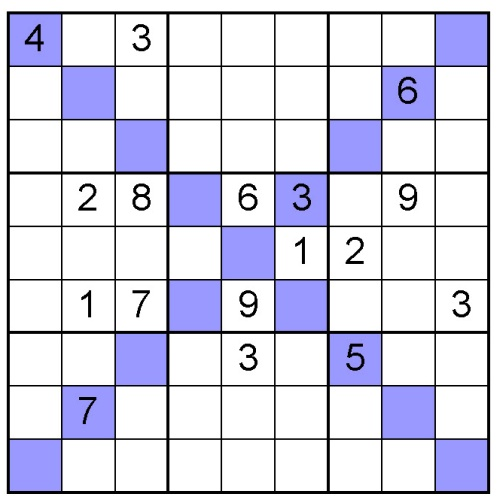
\includegraphics[scale=1.5]{Figures/sudokuX.jpg}
	\caption{Παράδειγμα ενός SUDOKU X παζλ. Οι δύο μεγάλες διαγώνιοι είναι σημειωμένες με μωβ χρώμα. Η κάθε μία πρέπει να περιέχει όλους τους αριθμούς από το 1 εως και το 9 ακριβώς μία φορα τον καθέναν.}
\end{figure}

Η μαθηματική μοντελοποίηση αυτής της παραλλαγής απαιτεί την προσθήκη επιπλέον περιορισμών που αντανακλούν τον επιπρόσθετο κανόνα που προαναφέραμε. Η μοντελοποίηση είναι όπως ορίστηκε στο κεφάλαιο 4.1 με την εξής προσθήκη στους περιορισμούς: \\

Για τη μία διαγώνιο του πίνακα:

\begin{align*}
	\sum_{r=1}^{n} x_{rrk} = 1 \quad k=1:9 \quad \text{μόνο ένα k στη διαγώνιο που ξεκινά από το κελι (1,1) και καταλήγει στο κελι (n,n)}
\end{align*}

και για την άλλη διαγώνιο του πίνακα:

\begin{align*}
\sum_{r=1}^{n} x_{r(n+1-r)k} = 1 \quad k=1:9 \quad \text{μόνο ένα k στη διαγώνιο που ξεκινά από το κελι (1,n) και καταλήγει στο κελι (n,1)}
\end{align*}

Συνεπώς, η τελική μαθηματική μοντελοποίηση για το SUDOKU X είναι:

\begin{align*}
	\begin{aligned}
		\min &\quad 0^{T}x \\
		\textup{s.t.}\quad
		\sum_{i=1}^{n}x_{ijk} = 1 &\quad j=1:n, \quad k=1:n \quad \text{μόνο ένα k σε κάθε στήλη του πίνακα} \\
		\sum_{j=1}^{n}x_{ijk} = 1 &\quad i=1:n, \quad k=1:n \quad \text{μόνο ένα k σε κάθε γραμμή του πίνακα} \\
		\sum_{j=mq-m+1}^{mq} {\sum_{i=mp-m+1}^{mp}x_{ijk}} = 1 &\quad k=1:n, \quad p=1:m, \quad q=1:m \quad \text{μόνο ένας ακέραιος k σε κάθε υποπίνακα} \\
		\sum_{k=1}^{n}x_{ijk} = 1 &\quad i=1:n, \quad j=1:n \quad \text{όλα τα κελιά του πίνακα πρέπει να συμπληρωθούν} \\
		\sum_{r=1}^{n} x_{rrk} = 1 &\quad k=1:9 \quad \text{μόνο ένα k στη διαγώνιο που ξεκινά από το κελι (1,1) και καταλήγει στο κελι (n,n)} \\
		\sum_{r=1}^{n} x_{r(n+1-r)k} = 1 &\quad k=1:9 \quad \text{μόνο ένα k στη διαγώνιο που ξεκινά από το κελι (1,n) και καταλήγει στο κελι (n,1)} \\
		x_{ijk} = 1 \forall (i,j,k) \in G &\quad \text{τα κελιά του πίνακα που είναι συμπληρωμένα είναι "on"} \\
		x_{ijk} \in {0,1}&
\end{aligned}
\end{align*}

\subsection{Four Square SUDOKU}

Το Four Square SUDOKU περιέχει τους κανόνες του κλασσικού SUDOKU και έναν επιπλέον κανόνα. Αν υποθέσουμε ότι αναφερόμαστε σε \(9 \times 9\) πίνακα, τότε στο Four Square SUDOKU δημιουργόυμε τέσσερις επιπλέον υποπεριοχές στον πίνακα μεγέθους \(3 \times 3\), όπως φαίνεται στο Figure 4.2. Στίς περιοχές αυτες πρέπει να περιέχονται όλοι οι ακέραιοι αριθμοί από το 1 ως το 9. \par 

\begin{mytheorem}{Four Square SUDOKU}{}
	Οι κανόνες για το Four Square SUDOKU σε έναν πίνακα μεγέθους \(9 \times 9\) με υποπίνακες μεγέθους \(3 \times 3\) είναι: \\
	\(\bullet\) Κάθε γραμμή του πίνακα μεγέθους 9 να περιέχει ακριβώς μια φορά κάθε ακέραιο αριθμό από το 1 ως το n. \\
	\(\bullet\) Κάθε στήλη του πίνακα μεγέθους 9 να περιέχει ακριβώς μια φορά κάθε ακέραιο αριθμό από το 1 ως το 9. \\
	\(\bullet\) Κάθε υποπίνακας μεγέθους \(3 \times 3\) να περιέχει ακριβώς μια φορά κάθε ακέραιο αριθμό από το 1 ως το 9. \\
	\(\bullet\) Κάθε υποπεριοχή μεγέθους
\(3 \times 3\) να περιέχει όλους τους ακέραιους από το 1 ως το 9. \\
\end{mytheorem}

\begin{figure}[h]
	\centering	
	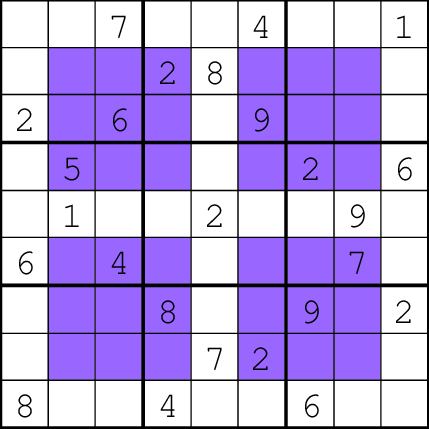
\includegraphics[scale=0.7]{Figures/An-example-Four-Square-Sudoku-puzzle.png}
	\caption{Παράδειγμα ενός Four Square SUDOKU παζλ. Οι τέσσερις περιοχές είναι σημειωμένες με μωβ χρώμα. Η κάθε μία πρέπει να περιέχει όλους τους αριθμούς από το 1 εως και το 9 ακριβώς μία φορα τον καθέναν.}
\end{figure}

Η μοντελοποίηση της συγκεκριμένης παραλλαγής SUDOKU απαιτεί την προσθήκη επιπλέον περιορισμών, που αποτυπώνουν τον τελευταίο κανόνα του Ορισμού 4.3.2. Οι επιλογές για τα i και j καθορίζουν τις υποπεριοχές. Οι περιορισμοί που δίνουμε στη συνέχεια αποτυπώνουν τις μωβ υποπεριοχές του Figure 4.2.\\

\begin{align*}
	\sum_{r=i}^{i+2}{\sum_{c=j}^{j+2}x_{rck}} = 1 \quad i=2,6; \quad j=2,6; \quad k=1:9
\end{align*}

Συνεπώς, η τελική μαθηματική μοντελοποίηση για το Four Square SUDOKU είναι:

\begin{align*}
	\begin{aligned}
		\min &\quad 0^{T}x \\
		\textup{s.t.}\quad
		\sum_{i=1}^{9}x_{ijk} = 1 &\quad j=1:9, \quad k=1:9 \quad \text{μόνο ένα k σε κάθε στήλη του πίνακα} \\
		\sum_{j=1}^{9}x_{ijk} = 1 &\quad i=1:9, \quad k=1:9 \quad \text{μόνο ένα k σε κάθε γραμμή του πίνακα} \\
		\sum_{j=3q-3+1}^{3q} {\sum_{i=3p-3+1}^{3p}x_{ijk}} = 1 &\quad k=1:9, \quad p=1:3, \quad q=1:3 \quad \text{μόνο ένας ακέραιος k σε κάθε υποπίνακα} \\
		\sum_{k=1}^{9}x_{ijk} = 1 &\quad i=1:9, \quad j=1:9 \quad \text{όλα τα κελιά του πίνακα πρέπει να συμπληρωθούν} \\
		\sum_{r=i}^{i+2}{\sum_{c=j}^{j+2}x_{rck}} = 1 &\quad i=2,6; \quad j=2,6; \quad k=1:9 \quad \text{οι επιπλέον υποπεριοχές πρέπει να περιέχουν όλους τους ακέραιους από το 1 ως το 9 ακριβώς μία φορά} \\
		x_{ijk} = 1 \forall (i,j,k) \in G &\quad \text{τα κελιά του πίνακα που είναι συμπληρωμένα είναι "on"} \\
		x_{ijk} \in {0,1}&
	\end{aligned}
\end{align*}

\subsection{Four Pyramids SUDOKU}

Η παραλλαγή Four Pyramids SUDOKU είναι παρόμοια με την Four Square SUDOKU παραλλαγή που αναφέραμε στην προηγούμενη υποενότητα, με τη διαφορά ότι εδώ οι επιπλέον υποπεριοχές του πίνακα στις οποίες πρέπει να περιέχονται όλοι οι ακέραιοι αριθμοί από το 1 ως το 9 ακριβώς μία φορά στην κάθε μία δεν έχουν πλέον τη μορφή τετραγώνων, αλλά τριγωνική μορφή.

\begin{mytheorem}{Four Pyramids SUDOKU}{}
	Οι κανόνες για το Four Pyramids SUDOKU σε έναν πίνακα μεγέθους \(9 \times 9\) με υποπίνακες μεγέθους \(3 \times 3\) είναι: \\
	\(\bullet\) Κάθε γραμμή του πίνακα μεγέθους 9 να περιέχει ακριβώς μια φορά κάθε ακέραιο αριθμό από το 1 ως το n. \\
	\(\bullet\) Κάθε στήλη του πίνακα μεγέθους 9 να περιέχει ακριβώς μια φορά κάθε ακέραιο αριθμό από το 1 ως το 9. \\
	\(\bullet\) Κάθε υποπίνακας μεγέθους \(3 \times 3\) να περιέχει ακριβώς μια φορά κάθε ακέραιο αριθμό από το 1 ως το 9. \\
	\(\bullet\) Κάθε υποπεριοχή μεγέθους
\(3 \times 3\) να περιέχει όλους τους ακέραιους από το 1 ως το 9. \\
\end{mytheorem}

\begin{figure}[h]
	\centering	
	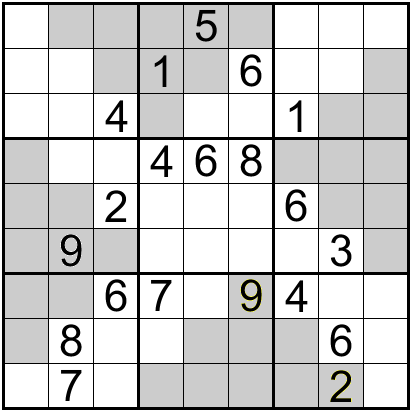
\includegraphics[scale=0.7]{Figures/Pyramid Sudoku.png}
	\caption{Παράδειγμα ενός Four Pyramids SUDOKU παζλ. Οι τέσσερις τριγωνικές περιοχές είναι σημειωμένες με γκρί χρώμα. Η κάθε μία πρέπει να περιέχει όλους τους αριθμούς από το 1 εως και το 9 ακριβώς μία φορα τον καθέναν.}
\end{figure}

Η μαθηματική μοντελοποίηση απαιτεί την προσθήκη των παρακάτων περιορισμών στη μοντελοποίηση του κλασσικού SUDOKU.

\begin{align*}
	\sum_{r=1}^{3}{\sum_{c=3+r}^{9-r} x_{rck}} = 1 \quad k=1:9 \\
	\sum_{c=1}^{3}{\sum_{r=1+c}^{7-c} x_{rck}} = 1 \quad k=1:9 \\\\
	\sum_{r=7}^{9}{\sum_{c=11-r}^{r-7} x_{rck}} = 1 \quad k=1:9 \\
	\sum_{c=7}^{9}{\sum_{r=13-c}^{c-1} x_{rck}} = 1 \quad k=1:9 \\	
\end{align*}

Οπότε, τελικά, η μαθηματική μοντελοποίηση για το Four Pyramids SUDOKU, αν απαριθμήσουμε τις πυραμίδες με τη φορά του ρολογιού, είναι:

\begin{align*}
	\begin{aligned}
		\min &\quad 0^{T}x \\
		\textup{s.t.}\quad
		\sum_{i=1}^{9}x_{ijk} = 1 &\quad j=1:9, \quad k=1:9 \quad \text{μόνο ένα k σε κάθε στήλη του πίνακα} \\
		\sum_{j=1}^{9}x_{ijk} = 1 &\quad i=1:9, \quad k=1:9 \quad \text{μόνο ένα k σε κάθε γραμμή του πίνακα} \\
		\sum_{j=3q-3+1}^{3q} {\sum_{i=3p-3+1}^{3p}x_{ijk}} = 1 &\quad k=1:9, \quad p=1:3, \quad q=1:3 \quad \text{μόνο ένας ακέραιος k σε κάθε υποπίνακα} \\
		\sum_{k=1}^{9}x_{ijk} = 1 &\quad i=1:9, \quad j=1:9 \quad \text{όλα τα κελιά του πίνακα πρέπει να συμπληρωθούν} \\
		\sum_{r=1}^{3}{\sum_{c=3+r}^{9-r} x_{rck}} = 1 &\quad k=1:9 \quad \text{η πρώτη πυραμίδα να έχει μόνο ένα k} \\
		\sum_{c=1}^{3}{\sum_{r=1+c}^{7-c} x_{rck}} = 1 &\quad k=1:9 \quad \text{η δεύτερη πυραμίδα να έχει μόνο ένα k}\\
		\sum_{r=7}^{9}{\sum_{c=11-r}^{r-7} x_{rck}} = 1 &\quad k=1:9 \quad \text{η τρίτη πυραμίδα να έχει μόνο ένα k} \\
		\sum_{c=7}^{9}{\sum_{r=13-c}^{c-1} x_{rck}} = 1 &\quad k=1:9 \quad \text{η τέταρτη πυραμίδα να έχει μόνο ένα k} \\
		x_{ijk} = 1 \forall (i,j,k) \in G &\quad \text{τα κελιά του πίνακα που είναι συμπληρωμένα είναι "on"} \\
		x_{ijk} \in {0,1}&
	\end{aligned}
\end{align*}

\subsection{Position SUDOKU}

Στην παραλλαγή Position SUDOKU εκτός από τους κανόνες του κλασσικού SUDOKU πρέπει να ικανοποιείται και ένα επιπλέον περιορισμός. Τα κελιά (1,1) σε όλους τους \(3 \times 3\) υποπίνακες πρέπει να περιέχουν όλους τους ακέραιους από το 1 ως το 9 ακριβώς μια φορά, αντίστοιχα τα κελιά (1,2) όλων των υποπινάκων κοκ. Οι κανόνες του Position SUDOKU συνοψίζονται στον παρακάτω ορισμό. \par 

\begin{mytheorem}{Position SUDOKU}{}
	Οι κανόνες για το Position SUDOKU σε έναν πίνακα μεγέθους \(9 \times 9\) με υποπίνακες μεγέθους \(3 \times 3\) είναι: \\
	\(\bullet\) Κάθε γραμμή του πίνακα μεγέθους 9 να περιέχει ακριβώς μια φορά κάθε ακέραιο αριθμό από το 1 ως το n. \\
	\(\bullet\) Κάθε στήλη του πίνακα μεγέθους 9 να περιέχει ακριβώς μια φορά κάθε ακέραιο αριθμό από το 1 ως το 9. \\
	\(\bullet\) Κάθε υποπίνακας μεγέθους \(3 \times 3\) να περιέχει ακριβώς μια φορά κάθε ακέραιο αριθμό από το 1 ως το 9. \\
	\(\bullet\) Κάθε κελί (i,j) με i=1:9 και j=1:9 σε όλους τους υποπίνακες \(3 \times 3\) να περιέχει ακριβώς μια φορά κάθε ακέραιο αριθμό από το 1 ως το 9.
\end{mytheorem}

\begin{figure}[h]
	\centering	
	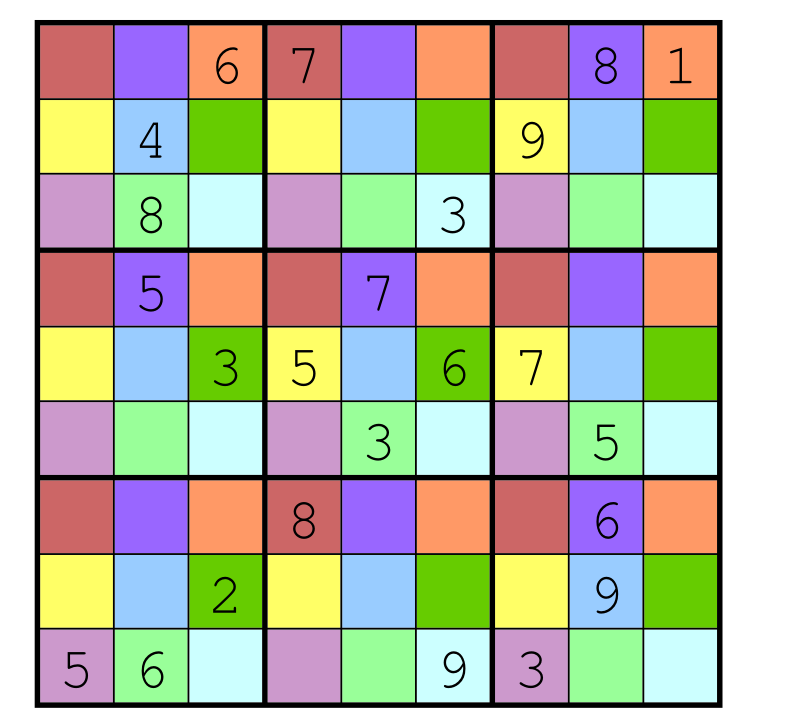
\includegraphics[scale=0.4]{Figures/positionSUDOKU.png}
	\caption{Παράδειγμα ενός Position SUDOKU παζλ. Κάθε κελί με το ίδιο χρώμα πρέπει να περιέχει όλους τους αριθμούς από το 1 εως και το 9 ακριβώς μία φορα τον καθέναν.}
\end{figure}

Η μαθηματική μοντελοποίηση θα περιλαμβάνει επιπλέον περιορισμούς, οι οποίοι δίνονται από τον πρακάτω τύπο: 

\begin{align*}
	\sum_{i=c}^{9}{\sum_{j=z}^{9} x_{ijk}} = 1 \quad c=1:(3):9 \quad j=1:(3):9 \quad \text{τα αθροίσματα προχωρούν με βήμα 3}
\end{align*}

Οπότε η τελική μορφή του προβλήματος βελτιστοποίησης είναι:

\begin{align*}
	\begin{aligned}
		\min &\quad 0^{T}x \\
		\textup{s.t.}\quad
		\sum_{i=1}^{9}x_{ijk} = 1 &\quad j=1:9, \quad k=1:9 \quad \text{μόνο ένα k σε κάθε στήλη του πίνακα} \\
		\sum_{j=1}^{9}x_{ijk} = 1 &\quad i=1:9, \quad k=1:9 \quad \text{μόνο ένα k σε κάθε γραμμή του πίνακα} \\
		\sum_{j=3q-3+1}^{3q} {\sum_{i=3p-3+1}^{3p}x_{ijk}} = 1 &\quad k=1:9, \quad p=1:3, \quad q=1:3 \quad \text{μόνο ένας ακέραιος k σε κάθε υποπίνακα} \\
		\sum_{k=1}^{9}x_{ijk} = 1 &\quad i=1:9, \quad j=1:9 \quad \text{όλα τα κελιά του πίνακα πρέπει να συμπληρωθούν} \\
		\sum_{i=c}^{9}{\sum_{j=z}^{9} x_{ijk}} = 1 &\quad c=1:(3):9 \quad j=1:(3):9 \quad k=1:9 \quad \text{κελιά με τις ίδιες συντεταγμένες σε όλους} \\ &\text{τους υποπίνακες έχουν μόνο ένα k} \\
		x_{ijk} = 1 \forall (i,j,k) \in G &\quad \text{τα κελιά του πίνακα που είναι συμπληρωμένα είναι "on"} \\
		x_{ijk} \in {0,1}&
	\end{aligned}
\end{align*}

\subsection{Three Magic SUDOKU}

Η παραλλαγή Three Magic SUDOKU υπάρχει ο επιπλέον κανόνας που ορίζει ότι στα σημειωμένα \(3 \times 3\) κουτιά (magic) οι 3 αριθμοί σε κάθε στήλη και οι 3 αριθμοί σε κάθε γραμμή αν αθροιστούν δίνουν το ίδιο αποτέλεσμα. Ένα παράδειγμα με 3 μαγικά κουτιά δίνεται στο Figure . Το πλήθος των μαγικών κουτιών μπορεί να ποικίλει. \par

\begin{mytheorem}{Three Magic SUDOKU}{}
	Οι κανόνες για το Three Magic SUDOKU σε έναν πίνακα μεγέθους \(9 \times 9\) με υποπίνακες μεγέθους \(3 \times 3\) είναι: \\
	\(\bullet\) Κάθε γραμμή του πίνακα μεγέθους 9 να περιέχει ακριβώς μια φορά κάθε ακέραιο αριθμό από το 1 ως το n. \\
	\(\bullet\) Κάθε στήλη του πίνακα μεγέθους 9 να περιέχει ακριβώς μια φορά κάθε ακέραιο αριθμό από το 1 ως το 9. \\
	\(\bullet\) Κάθε υποπίνακας μεγέθους \(3 \times 3\) να περιέχει ακριβώς μια φορά κάθε ακέραιο αριθμό από το 1 ως το 9. \\
	\(\bullet\) Σε κάθε μαγικό κουτί το άθροισμα των στηλών και των γραμμών πρέπει να είναι το ίδιο.
\end{mytheorem}

\begin{figure}[h]
	\centering	
	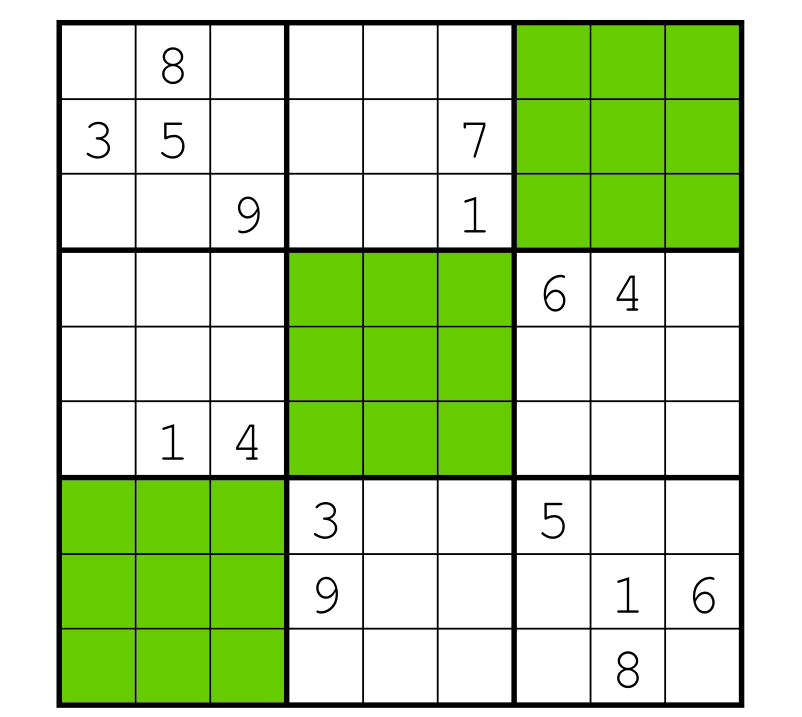
\includegraphics[scale=0.4]{Figures/threemagicSUDOKU.png}
	\caption{Παράδειγμα ενός Three Magic SUDOKU παζλ. Οι 3 αριθμοί σε κάθε στήλη και οι 3 αριθμοί σε κάθε γραμμή στα πράσινα \(3 \times 3\) κουτιά πρέπει αν προτεθούν να δίνουν τον ίδιο αριθμό.}
\end{figure}

Η μαθηματική μοντελοποίηση του Three Magic SUDOKU απαιτεί τον επιπλέον περιορισμό:

\begin{align*}
	...............
\end{align*}

Οπότε η τελική μορφή του προβλήματος βελτιστοποίησης είναι:

\begin{align*}
	\begin{aligned}
		\min &\quad 0^{T}x \\
		\textup{s.t.}\quad
		\sum_{i=1}^{9}x_{ijk} = 1 &\quad j=1:9, \quad k=1:9 \quad \text{μόνο ένα k σε κάθε στήλη του πίνακα} \\
		\sum_{j=1}^{9}x_{ijk} = 1 &\quad i=1:9, \quad k=1:9 \quad \text{μόνο ένα k σε κάθε γραμμή του πίνακα} \\
		\sum_{j=3q-3+1}^{3q} {\sum_{i=3p-3+1}^{3p}x_{ijk}} = 1 &\quad k=1:9, \quad p=1:3, \quad q=1:3 \quad \text{μόνο ένας ακέραιος k σε κάθε υποπίνακα} \\
		\sum_{k=1}^{9}x_{ijk} = 1 &\quad i=1:9, \quad j=1:9 \quad \text{όλα τα κελιά του πίνακα πρέπει να συμπληρωθούν} \\
		........ \\
		x_{ijk} = 1 \forall (i,j,k) \in G &\quad \text{τα κελιά του πίνακα που είναι συμπληρωμένα είναι "on"} \\
		x_{ijk} \in {0,1}&
	\end{aligned}
\end{align*}

\chapter{Δημιουργία SUDOKU παζλ}

Στο κεφάλαιο αυτό θα αναφερθούμε στους τρόπους με τους οποίους μπορούμε να δημιουργήσουμε SUDOKU παζλ. Αναλύουμε τη απλή bruteforce μέθοδο κι έπειτα συζητάμε τη δημιουργία παζλ από προγενέστερα παζλ.

\subsection{Δημιουργία SUDOKU παζλ με bruteforce}

Μία πρώτη προσέγγιση για τη δημιοργία ενός παζλ SUDOKU είναι το bruteforce. Σε έναν πίνακα μεγέθους \(n \times n\) τοποθετούμε τυχαία αριθμούς από το 1 ως το n στα κελιά του και στη συνέχεια ελέγχουμε αν ο τελικός πίνακας που προκύπτει συμμορφώνεται με τους κανόνες που αναφέρονται στον Ορισμό 5.3.1. \par

Η τεχνική αυτή δημιουργεί περίπου \(n^{n^2}\) διαφορετικούς πίνακες. Αν αναφερόμαστε σε πίνακα μεγέθους \(9 \times 9\), τότε ο αριθμός αυτός προσεγγίζει τους \(1.97\times10^{77}\) διαφορετικούς πίνακες. \par 

Το ερώτημα είναι πόσοι από αυτούς τους πίνακες συμμορφώνονται με τους κανόνες του Ορισμού 5.3.1. \par

Από το \cite{6} γνωρίζουμε ότι τα \(9 \times 9\) Latin squares είναι \(5.525\times10^27\) το πλήθος και αφού τα κλασσικά SUDOKU είναι ειδικές περιπτώσεις των Latin squares, ο αριθμός τους θα είναι μικρότερος από \(5.525\times10^27\). Τελικά, ο αριθμός των κλασσικών παζλ υπολογίστηκε στο \cite{7} το 2005 να είναι περίπου \(6.67\times10^21\). Αν ληφθούν υπόψη και οι συμμετριές, τότε ο αριθμός μειώνεται αισθητά \cite{8}.

Αν υποθέσουμε ότι ξεπερνάμε τους μεγάλους αριθμούς διαφορετικών πινάκων και σταματάμε την αναζήτηση valid πίνακα με το που βρούμε τον πρώτο. Είναι σημαντικό να γνωρίζουμε ποιος είναι ο ελάχιστος αριθμός δεδομένων κελιών (τα κελιά που περιέχουν αριθμούς στη αρχή), ώστε να καταφέρει ο παίκτης με βάση αυτά να φτάσει στη μοναδική λύση. Σε γενικές γραμμές δεν υπάρχει θεωρητική προσέγγιση που να απαντά σε αυτό το ερώτημα πλήρως, παρά μόνο πειραματικές προσεγγίζεις. Σίγουρα, οι πειραματικές προσεγγσεις υποδεικνύουν ότι χρειάζονται τουλάχιστον 17 κελιά συμπληρωμένα. Φυσικά, όσα περισσότερα δεδομένα κελιά δίνονται, τόσο πιο εύκολο γίνεται το παζλ. Η δυσκολία επίλυσης ενός παζλ καθορίζεται και από τη θέση των δεδομένων κελιών, αλλά και των τιμών που παίρνουν τα δεδομένα κελιά.

\subsection{Δημιουργία SUDOKU παζλ από προγενέστερα παζλ}

\pagebreak

\begin{thebibliography}{99}
	\bibitem[HG]{1}
	Howard Garns, 
	\url{https://en.wikipedia.org/wiki/Howard_Garns} \\
	
	\bibitem[BILP]{2}
	Binary Integer Programming and its Use for EnvelopeDetermination,
	Vladimir Y. Lunin, Alexandre Urzhumtsev, Alexander Bockmayr \\
	
	\bibitem[IPMS]{3}
	An Integer Programming Model for the Sudoku Problem,
	Andrew C. Bartlett,	Timothy P. Chartier, Amy N. Langville, Timothy D. Rankin,
	3 Μάη 2008 \\
	
	\bibitem[SATPR]{4}
	Τεχνητή Νοημοσύνη Μία σύγχρονη προσέγγιση, Δεύτερη Αμερικανική έκδοση, εκδόσεις Κλειδάριθμος,
	Stuart Russell, Peter Norvig,
	ISBN: 960-209-873-2,
	Κεφάλαιο 5 Προβλήματα Ικανοποίησης Περιορισμών, σελ.:179,180,181 \\
	
	\bibitem[HPS]{5}
	Human Problem Solving: Sudoku Case Study,
	Radek Pelánek,
	Ιανουάριος 2011 \\

	\bibitem[LAT]{6}
	The number of \(9 \times 9\) Latin squares, Discrete Mathematics,
	Stanley Bammel and Jermome Rothstein,
	1975 \\

	\bibitem[FEL]{7}
	There are 6670903752021072936960 Sudoku grids,
	Bertram Felgenhauer and Frazer Jarvis,
	\url{ http://www.afjarvis.staff.shef.ac.uk/sudoku/}//

	\bibitem[RJ]{8}
	There are 5472730538 essentially different Sudoku grids . . . and the
Sudoku symmetry group,
	Ed Russell and Frazer Jarvis,
	\url{ http://www.afjarvis.staff.shef.ac.uk/sudoku/sudgroup.html/}//

\end{thebibliography}

\end{document}
